%!TEX root = /Users/smsohan/Taggy/Thesis/ucalgthes1_root_0.tex
\fancyhead[RO,LE]{\thepage}
\fancyfoot{} 
\chapter{TAGGY}
These chapter is dedicated to the implementation details of Taggy. First the underlying assumptions behind Taggy are discussed. Then, a definition of the adapted agile project context is given. With this background information, a high level architecture of Taggy is explained. Next, the workflow of auto-tagging is discussed. The mathematical and algorithmic details are provided in the similarity computation section. This chapter also includes the details about the software frameworks used to implement Taggy. Finally, an illustrative example is given to explain Taggy in action.

\section{Assumptions}
Taggy is designed based on the following assumptions to auto-tag the emails with user stories:

\begin{enumerate}
	\item An email is potentially relevant to a user story when:
		\begin{itemize}
			\item It is sent during the iteration time frame of the user story. Since agile projects are developed in small iterations and the core concentration during an iteration is to deliver the user stories from the iteration backlog, it is highly likely that the email conversation will be about the user stories from current iteration backlog. However, it is also possible to see some conversations about near past or near future iteration backlogs. Such conversation are mainly used to provide post-delivery feedback and collaborate about upcoming work. Taggy uses this assumption to shorten its search space for relevant user stories by filtering out the ones from far past.
			
			\item The developers and/or customers of a user story participate in the email. For an example, if Alex (a developer) is working on a user story for Jane (the customer), and Alex writes an email to Jane, they are more likely to discuss about the user story than Peri (another developer) and Jane. However, Peri can always participate in a discussion about Alex's work in an agile team, where open communication is encouraged. But, it is highly unlikely that two people who are neither assigned developers or customers of a user story will write emails about that. This assumption about people's participation in email provides an important context in Taggy's similarity computation.
			
			\item There is a minimum degree of text similarity between an email and a user story. An email has text in terms of its subject, body and attachments. Although not explicit, it is likely that such text in the emails will show some relevance to the user stories. This may not be true in all cases, especially if there is a lot of face-to-face communication. However, this is not the case for in distributed projects with huge time zone difference. Taggy computes a text similarity between the email and user story and discards the ones that show very poor match.
		\end{itemize}
	 \item A web-based project management tool is used to manage the distributed agile project. To automatically link up emails with user stories, Taggy looks into this tool for information about user stories. This assumption is required because if teams only use volatile physical artifacts, such as sticky notes for user stories on a whiteboard, it is not possible to automatically find the user stories. As discussed in literature review, distributed agile teams use a number of different types of such tools.
	
	\item The project management tool captures user stories with its planning information including a) assigned developers, b) customer and c) iteration timeframe. The presence of this planning information is essential as it serves the meta data that is necessary to auto-tag emails. While it is generally expected that this data be available, it is not required that each and every user story contains all the required planning information. Since Taggy uses context alongside text similarity, having the context helps in making a more informed decision in auto-tagging.
	
	\item Each project has its own email address so that when people are sending emails about a project to someone, they can keep the project's email in the copy. This serves as the input to Taggy for auto-tagging. Also, giving every project a unique email address ensures Taggy can correctly determine the target project for an email. Since most people who use email are already familiar with the CC: feature, this adds little learning curve or communication overhead. It is assumed that indicating the project in CC: serves a convenient input mechanism compared to manually copy-pasting the email contents into a system for every useful email.		
	
	\item The subject of an email carries an important clue about its relationship with a user story. Although, subject is just a text similar to body or attachment contents of an email, due to professional etiquette and for the sake of grabbing attention, people write revealing subject while writing emails about projects. Taggy distinguishes the text relevance of the subject from the rest of the email contents based on this assumption.
\end{enumerate}



\section{The Agile Project Context}
Taggy uses two kinds of context information that are available for agile user stories, namely Temporal context and People context. These contexts are defined below:

\begin{enumerate}
	\item \textbf{Temporal Context.} User stories in agile projects are grouped by small iterations so that a bunch of new user stories are potentially deliverable at the end of each iteration. These iterations are confined within specific start and end dates. This time-box works as the temporal context for a user story. For example, if a user story is developed during Iteration\#2, June 1 to June 14, then Taggy assumes people are more likely to write emails about the user story within this period than in the far past or future.
	
	\item \textbf{People context.} The people context for a user story is formed by its assigned developers and customers. A user story may have one or more customers, who are mainly responsible for providing the details proactively and also as questions arise during implementation. On the other hand, a user story is broken down into tasks and assigned to developers, testers and other technical team members. Taggy uses all these people relevant to a user story as its people context. For example, if an email is exchanged among the people in a user story, then Taggy puts a higher similarity rank than when the people context is different. The identification of the people context is done based on email addresses.
\end{enumerate}

Since Taggy combines context similarity with text similarity, the above contexts provide more confidence in auto-tagging. However, when some or all of the context information are missing for a user story, Taggy still applies whatever information is available to auto-tag emails with user stories.

\section{High Level Workflow}
Now that the assumptions and definitions of important terms are discussed, the Figure~\ref{fig:} shows the two main steps involved in the process of auto-tagging an email with user stories. Essentially as with most other machine learning techniques, Taggy needs to learn the important parameters before making decisions. Once the learning is done, Taggy uses the learned parameters to auto-tag emails.

%TODO: figure with description
As seen on Figure~\ref{fig:}, the learning process involves several iterations. Since the similarity computation uses multiple components, the learning process needs to address the importance of each component relative to others. To achieve this, first it produces an initial weight for the components and then learns the relative weights based on the training data. The details about learning is discussed later in Section X.

Once learned, Taggy can be used to auto-tag emails with user stories. This process is supposed to be in a live system as illustrated in Figure~\ref{fig:}
%TODO: figure with description

As discussed in assumptions, Taggy contains the user stories with planning information. Next, it follows the steps as shown in Figure~\ref{fig:} to complete the auto-tagging of emails against the saved user stories.

\begin{enumerate}
	\item \textbf{Copy emails to project mail address.} This is the input step for Taggy. As discussed in assumptions, Taggy identifies each project by its own email address. So, whenever someone sends an email about a project, they put the ``project email'' in the CC:. This is the only change in the business process that needs to be implemented by the distributed team. This intake process was successfully adapted in a previous work \cite{where_did_you}. In case someone forgets to do this while sending the email, it is possible to simply forward the email to ``project email'' later.
	
	\item \textbf{Grab email.} One the project related emails reach the inbox of ``project email'', Taggy picks up the email. It is common for email servers to allow access via POP or IMAP protocol. Taggy uses POP3 to read all incoming emails, including the attachments, if any. This grabbing runs on a background process, which can be scheduled to check for new emails in desired intervals. However, this email grabbing step can make use of any other email transfer protocol.

	\item \textbf{Save email.} After grabbing, Taggy saves the email into its database keeping a link to its project. After this step, even if auto-tagging fails, the email is stored in a shared place with the user stories. This step makes an email available for search and browsing without the need for looking into other's inbox.
	
	\item \textbf{Filter.} To auto-tag the email just grabbed, Taggy first reduces its search space by discarding the user stories of a project that were done in the far past or scheduled to be developed in the far future. This filtering process essentially finds the current iteration of the project, if any. Then considers the user stories from the current iteration and its neighboring iterations as potential candidates for auto-tagging the emails.

	\item \textbf{Compute local similarity.} In the reduced search space, Taggy computes local similarities for people and temporal contexts as well as separate text similarities for subject and body. The details of these local similarity computations are shown in equations x, y, z, w. 
	
	\item \textbf{Compute global similarity.} Next, for each of the user stories the similarity values from previous step are combined to produce a global similarity score. This computation is done based on the formula presented at equation x. This global similarity assigns a numeric value of the relative relevance between a user story and the email.
	
	\item \textbf{Sort.} The user stories are then sorted descendingly according to their global similarity value from previous step. This produces a list of user stories with the potentially most relevant user story at the top.
	
	\item \textbf{Pick.} Next, Taggy picks the user stories having global similarity scores above a predefined threshold. Having a threshold ensures Taggy only picks the ones that show sufficient relevance based on its learning. However, this also means, for some emails no user story may be picked.
	
	\item \textbf{Auto-tag.}	Finally, Taggy auto-tags the email with the picked user stories from the last step. This step adds database level links between the email and the user stories to be auto-tagged.
\end{enumerate}

However, to auto-tag instant messages, first three of the aforementioned steps differ significantly. The following the steps are used for the intake process of instant messages:

\begin{enumerate}
	\item \textbf{Activate instant message plugin.} Instant message clients often allow the use of plugins. For example, Skype \cite{skype} has a plugin framework and Taggy has a plugin for Skype. To input the instant messages, one needs to activate the Taggy plugin and select the project under discussion. Then, as the chat messages are exchanged, the plugin sends out the messages to Taggy over a web-based service. Typically the instant message clients provide meta data such as unique identification of a chat session, its individual messages, people and also the time stamp.

	\item \textbf{Grab instant message.} Taggy exposes a web service for the intake of instant messages. As soon as it finds a chat message from the plugin, it identifies the conversation based on the meta data.
	
	\item \textbf{Save instant message.} Taggy extracts out the context from an instant message and saves it in the database. For example, it matches the instant message identifier for people that are already stored in the database against the ones participating on a chat session. Also, it keeps track of the time stamp. As a result, an instant message is stored with a similar people and temporal context as that of an email. Taggy stores the content of different instant messages together as a session that belong to a single conversation as per the instant messenger.
\end{enumerate}

Since instant messages don't capture any subject, Taggy cannot produce a text similarity for this field. As a work around of this limitation, Taggy can be trained differently for instant messages where the contribution of subject similarity is ignored.

On a live system, as like any other machine learning solution, Taggy cannot discard the possibility of a wrong auto-tagging decision. When someone spots such a faulty auto-tagging in Taggy, she can manually correct it.

\section{Architecture}
Taggy is composed of a number of different components to support the workflow as outlined in the previous section. The architecture of Taggy is depicted at Figure~\ref{fig:architecture}. Next, the details about each component from the figure is discussed following a bottom-up approach.

\begin{figure*}[bt]
	\centering
	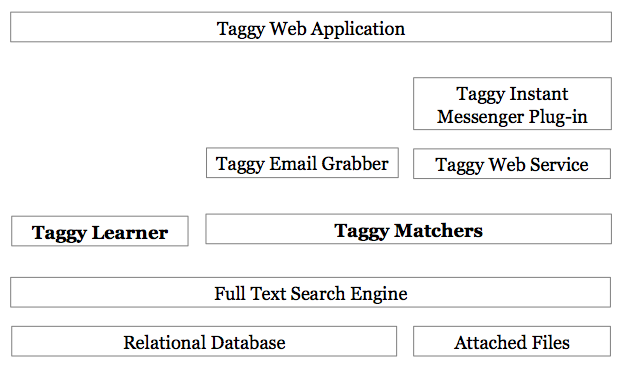
\includegraphics[width=\textwidth]{Architecture.png}
    \caption{Taggy Components}
	\label{fig:architecture}
\end{figure*}

\begin{enumerate}
	\item \textbf{Relational Database.} This relational database component persists the agile project related information. To address the concern of auto-tagging, this database keeps the following information:
		\begin{itemize}
			\item People. People information includes the name, email address and instant messenger id, if any. Also, a project vs. people mapping is stored.
			\item Iteration. Iterations, defined by start and end dates, are also saved.
			\item User story. Each user story may have a title and description. Also, if the story is planned, then information about its iteration and assigned people are stored in the database.
			\item Email. The database also stores the subject and content of the emails with a link to sender and recipients if they are found in the people information. If the email is tagged with a user story, then this information is kept in the database as well.
			\item Instant Message. Similar to emails, the database stores the instant messages and their tagging information.
		\end{itemize}

	 \item \textbf{Attached Files.} Attached Files is a simple file system storage where all attachments are kept. An attachment may be part of a user story definition or can be extracted from an email.
	
	 \item \textbf{Full Text Search Engine.} This component produces full text index from contents found in user stories, emails and their associated attachments. This is a third party component that can handle synonyms and language specific stems. The attached files are only indexed for full text search if it is meaningful, for example image files are not indexed where PDF file contents are.
	
	\item \textbf{Taggy Matchers.} This is the core component of Taggy that produces the auto-tagging, i.e. the similarity related computations are done inside this component. There are two matchers inside Taggy for now: email matcher and instant message matcher. These two matchers share some common computation logic. However, instant messages don't have subjects as found in emails and as a result, the two matchers use different relative weights and minimum threshold similarity scores to auto-tag. The matchers depend on the full text search engine and the relational database to lookup for required data.
	
	\item \textbf{Taggy Learner.} As discussed before, Taggy requires training to learn the different parameters. This component takes care of the learning process. During learning the Learner uses the Matcher to auto-tag an email and depending on the outcome, it may learn the parameters of interest. Once the learning is complete, the learner sets the relative weights to be used in the Matcher. So, the core part of auto-tagger is a mix of its Learner and Matcher components.
	
	\item \textbf{Taggy Email Grabber.} The Email Grabber component works as a background process that periodically checks for incoming emails in any of the project emails. If it finds one, it reads the email, saves a copy in the relational database as well as downloads the attachments into Attached Files. Next, the text contents are all indexed through the Full Text Search Engine. With this data persisted, it invokes the Matcher component to auto-tag the email against the relevant user stories. This handles the email intake process to Taggy.
	
	\item \textbf{Taggy Web Service.} Taggy exposes a web-service so that an instant messenger plugin can push instant messages into Taggy.
	
	\item \textbf{Taggy Instant Messenger Plug-in.} This component is installed as a plug in to an instant messenger. Once activated, this component sends instant messages to the Web Service Component.
	
	\item \textbf{Taggy Web Application.} The web application provides interfaces for manipulating everything in Taggy. For example, one can browse a user story and see all related emails and instant messages or vice versa. Also, one can search through all the contents, including the attachments. In a nutshell, this is a light-weight agile project management tool with the additional feature that it auto-tags emails and instant messages.
\end{enumerate}






\section{Similarity Computation}
	\subsection{Similarity Function}
	\subsection{Learning Relative Weights}	
	\subsection{Email Matching}
	\subsection{Instant Message Matching}
\section{Implementation Details}
\section{An Illustrative Example}	
